\chapter{Client}
\label{ch:client}
Das nachfolgende Kapitel beschreibt die Entwicklung einer Applikation, welche die in Kapitel~\ref{ch:neuronalesNetz}
ab Seite~\pageref{ch:neuronalesNetz} implementierte Architektur nutzt um Anfragen an die neuronalen Netze einfacher
und schöner zu gestalten.

Dabei ist die Anwendung für die Eingabe der Parameter zuständig und das Abfangen von falsch eingetragenen Werten in
das Formular. Anschließend ist die Übertragung der Werte an die neuronalen Netze möglich und die Vorhersagen werden
aufbereitet dargestellt.

Die Architektur beherbergt zwar zwei Anwendungen mit jeweils einem Endpunkt, allerdings sind diese gemeinsam über
den API Connect Service aufrufbar. Dies erleichtert die Entwicklung der Anwendung dahingehend, dass lediglich eine
Kommunikation zwischen der neuen Applikation und dem Bluemix-Service notwendig ist.

Da, wie in~\cite{online_client_apps} zu lesen, Smartphone-Apps eine immer wichtigere Rolle im Leben spielen, soll neben
einer Webanwendung (englisch Frontend) auch für die beiden größten Hersteller von Smartphone-Betriebssystemen eine App
entstehen. Somit kann ein noch viel größerer Kundenbereich abgedekt werden.

Das Frontend soll in einem Container laufen um ihn möglichst schnell und komfortabel sowohl in der Cloud als auch 
im eigenen Rechenzentrum betreiben zu können. In Abbilung~\ref{fig:schematische_architektur_4} auf 
Seite~\pageref{fig:schematische_architektur_4} zeigt die schematische Architektur des Frontends mit den ausgehenden
Anfragen.

Die notwenigen Schritte für den Aufbau eines Containers sollen in einem Continuous Deployment verankert werden, um sie
möglichst Modular zu halten.

\begin{figure}[h]
    \centering
    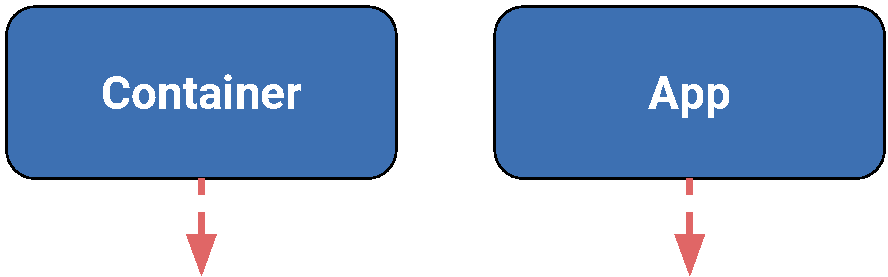
\includegraphics[scale=0.5]{images/kapitel_4/architektur_schematisch.pdf}
    \caption{Schematische Darstellung der Architektur}
    \label{fig:schematische_architektur_4}
\end{figure}